\documentclass{article}
\usepackage{amsmath}
\usepackage[utf8]{inputenc}
\usepackage{natbib}
\usepackage{graphicx}


\title{LELEC2103 : Labview6}
\author{Bronchain Olivier \\ Schellekens Vincent \\ group 7}
\date{\today}

\begin{document}

\maketitle
\section{Frequency selectivity of wireless channels}
\subsection{Symbol rate}
For the narrowband channel (sample rate = $4MSample/s$, oversample factor = $20$), the symbol rate is given by : 
\begin{equation}
\frac{4MSample/s}{20}*\frac{1}{64} = 3125 Symbols/s
\end{equation}

where 64 is the size of the FFT (or the number of symbols sent at the same time). The symbol period in OFDM modulation is thus 64 times larger than for a "classical" modulation using the same sample rate and oversample factor. For the wideband channel (sample rate = $20Msample/s$, oversample factor = $4$), we similarly obtain : 
\begin{equation}
\frac{20MSample/s}{4}*\frac{1}{64} = 78125 Symbols/s
\end{equation}

We see that the symbol rate is much higher for the wide-band channel, which corresponds to our intuition. 

The effective channel length is $5E-7s$ for the narrowband channel and $1E-7s$ for the wideband channel, as can be derived from the power delay profiles figure \ref{effL}. The channel length is greater for the narrowband channel.

    
\begin{figure}[h!]
    \centering
    \begin{tabular}{c c}
     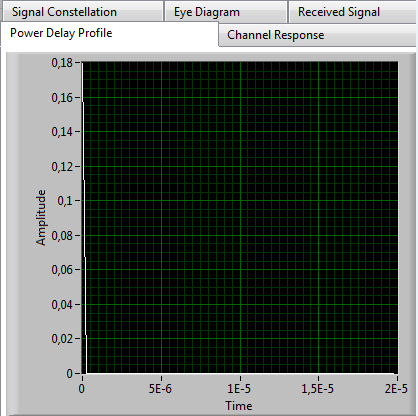
\includegraphics[width = 0.4 \textwidth ]{narrowT} & 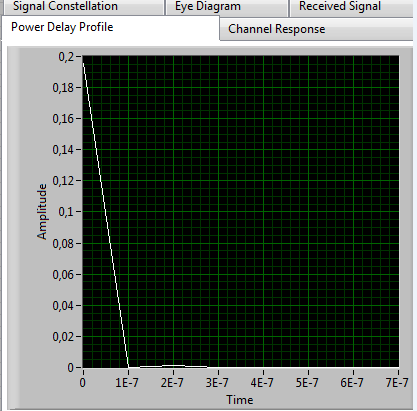
\includegraphics[width = 0.4 \textwidth]{wideT} \\
    \end{tabular}
    \caption{Left : power delay profile for narrowband channel; right : for the wideband channel}
    \label{effL}
\end{figure}
    
The narrowband channel is flat; that can be verified by inspecting figure \ref{narrowflat} that shows the frequency response for the narrowband channel. This channel is thus not frequency selective. For the wideband channel on the other hand, the channel is frequency selective.

\begin{figure}[h!]
    \centering
    \begin{tabular}{c c}
     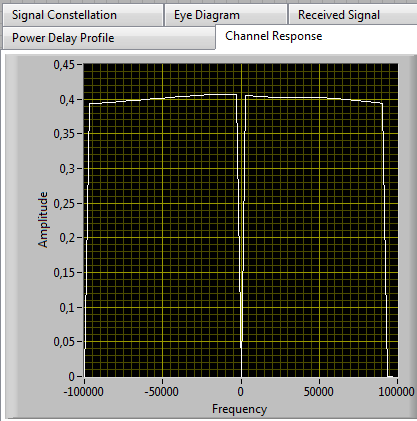
\includegraphics[width = 0.4 \textwidth ]{narrowRep} & 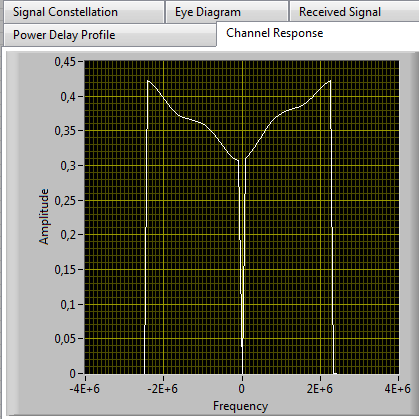
\includegraphics[width = 0.4 \textwidth]{wideRep} \\
    \end{tabular}
    \caption{Left : channel frequency response for narrowband channel; right : for the wideband channel}
    \label{narrowflat}
\end{figure}
    
To show that when $L_h = 0$ the channel is necessarily flat, we simply compute $H[k]$ by applying the DFT definition : 

\begin{equation}
H[k] = \sum_{l=0}^{L} h[l] e^{-j2 \pi kl/N} = h[0]e^{-j2 \pi k0/N} + 0 = h[0] \: \forall k
\end{equation}
We see that the DFT of the channel impulse response is a constant. What happens if $L_h > 0$? To show that the channel becomes frequency selective, it is sufficient to show that $\exists k_1,k_2$ such that $H[k_1] \neq H[k_2]$ : we can take $k_1 = 0$ and $k_2 = N/2$ for example (assuming N is even, but many other choices are possible). We get :

\begin{equation}
H[0] = \sum_{l=0}^{L} h[l] \textsf{ and } H[N/2] = \sum_{l=0}^{L} (-1)^{l} h[l] 
\end{equation}
it is trivial that those values are, in the general case, not equal to each other.

\section{Sensitivity to Frequency offset}
    The OFDM is sensitive to frequency offset. The influence of frequency offset in a OFDM modulation is equivalent to the influence of delay on a single carrier modulation. \\
    In single carrier modulation not sampling at the exact time cause the sample to not have the wanted phase. This is exactly the same in OFDM modulation but in the frequency domain. The symbols aren't perfectly recovered because of the frequency offset. This can be shown in Figure \ref{compare}. To conclude, where we had inter-symbol interference before, we now have inter-carrier interference.
    \begin{figure}[h!]
    \centering
    \begin{tabular}{c c}
     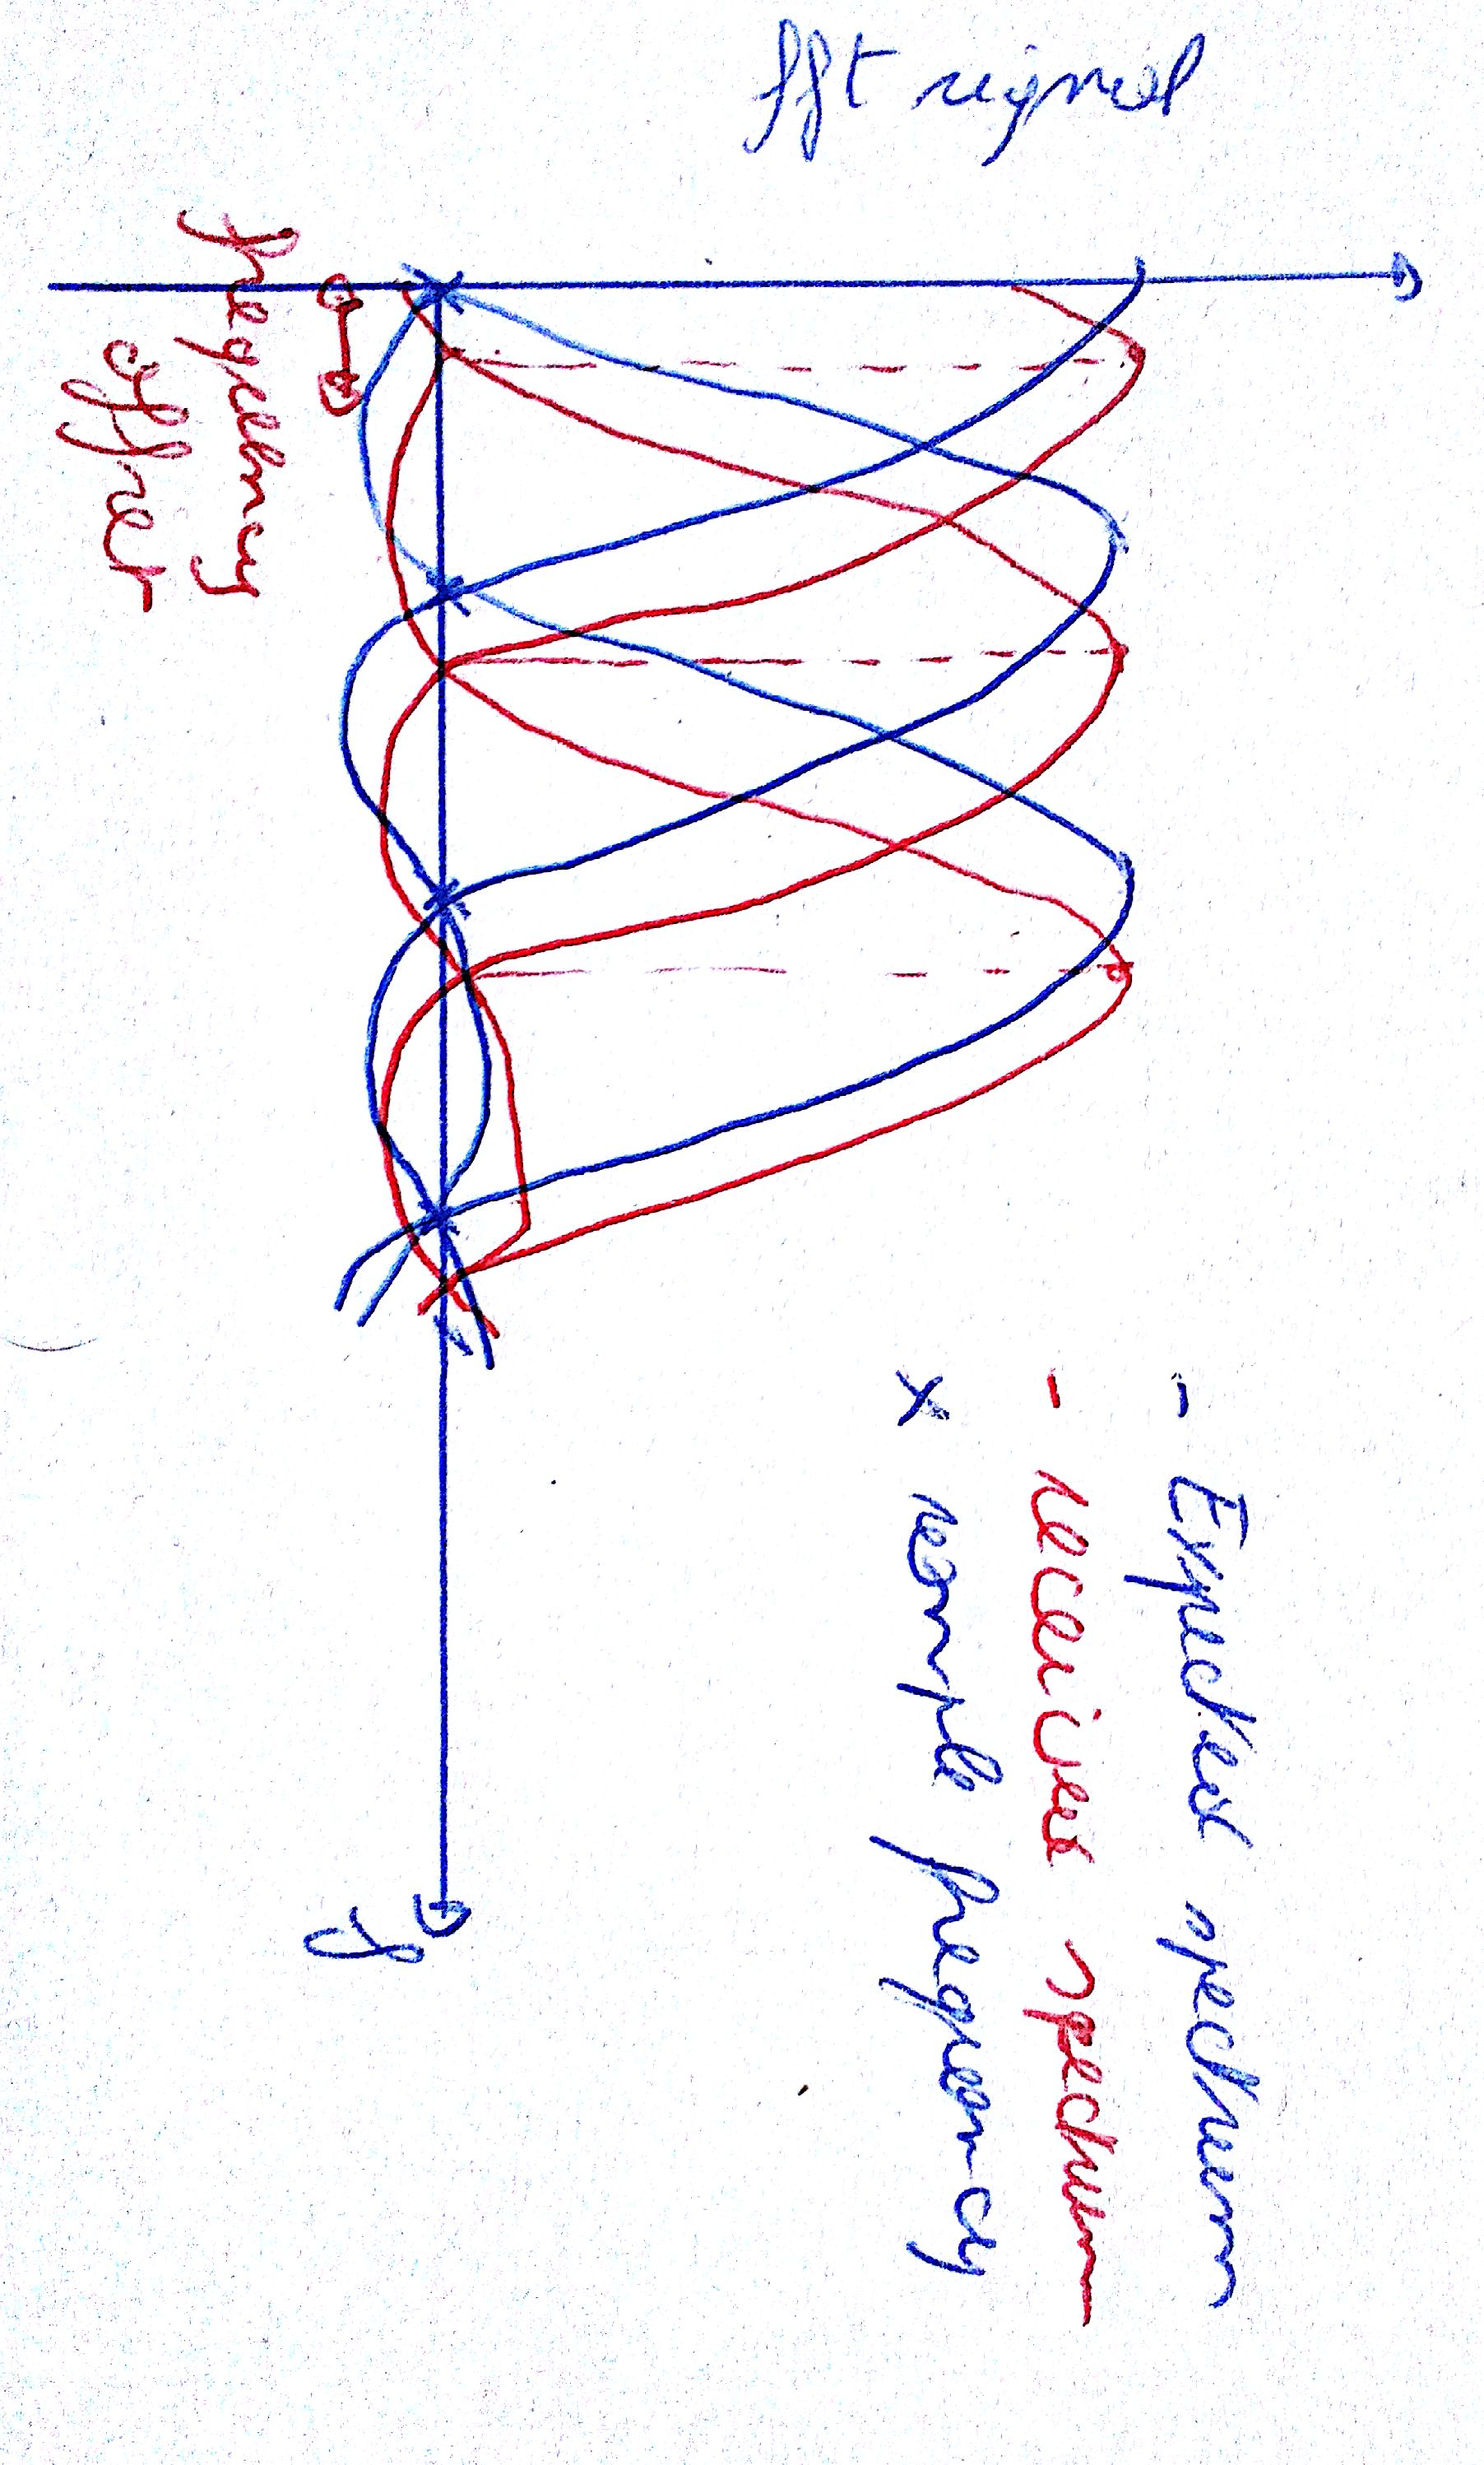
\includegraphics[width = 0.3 \textwidth , angle=90]{time.jpg} & 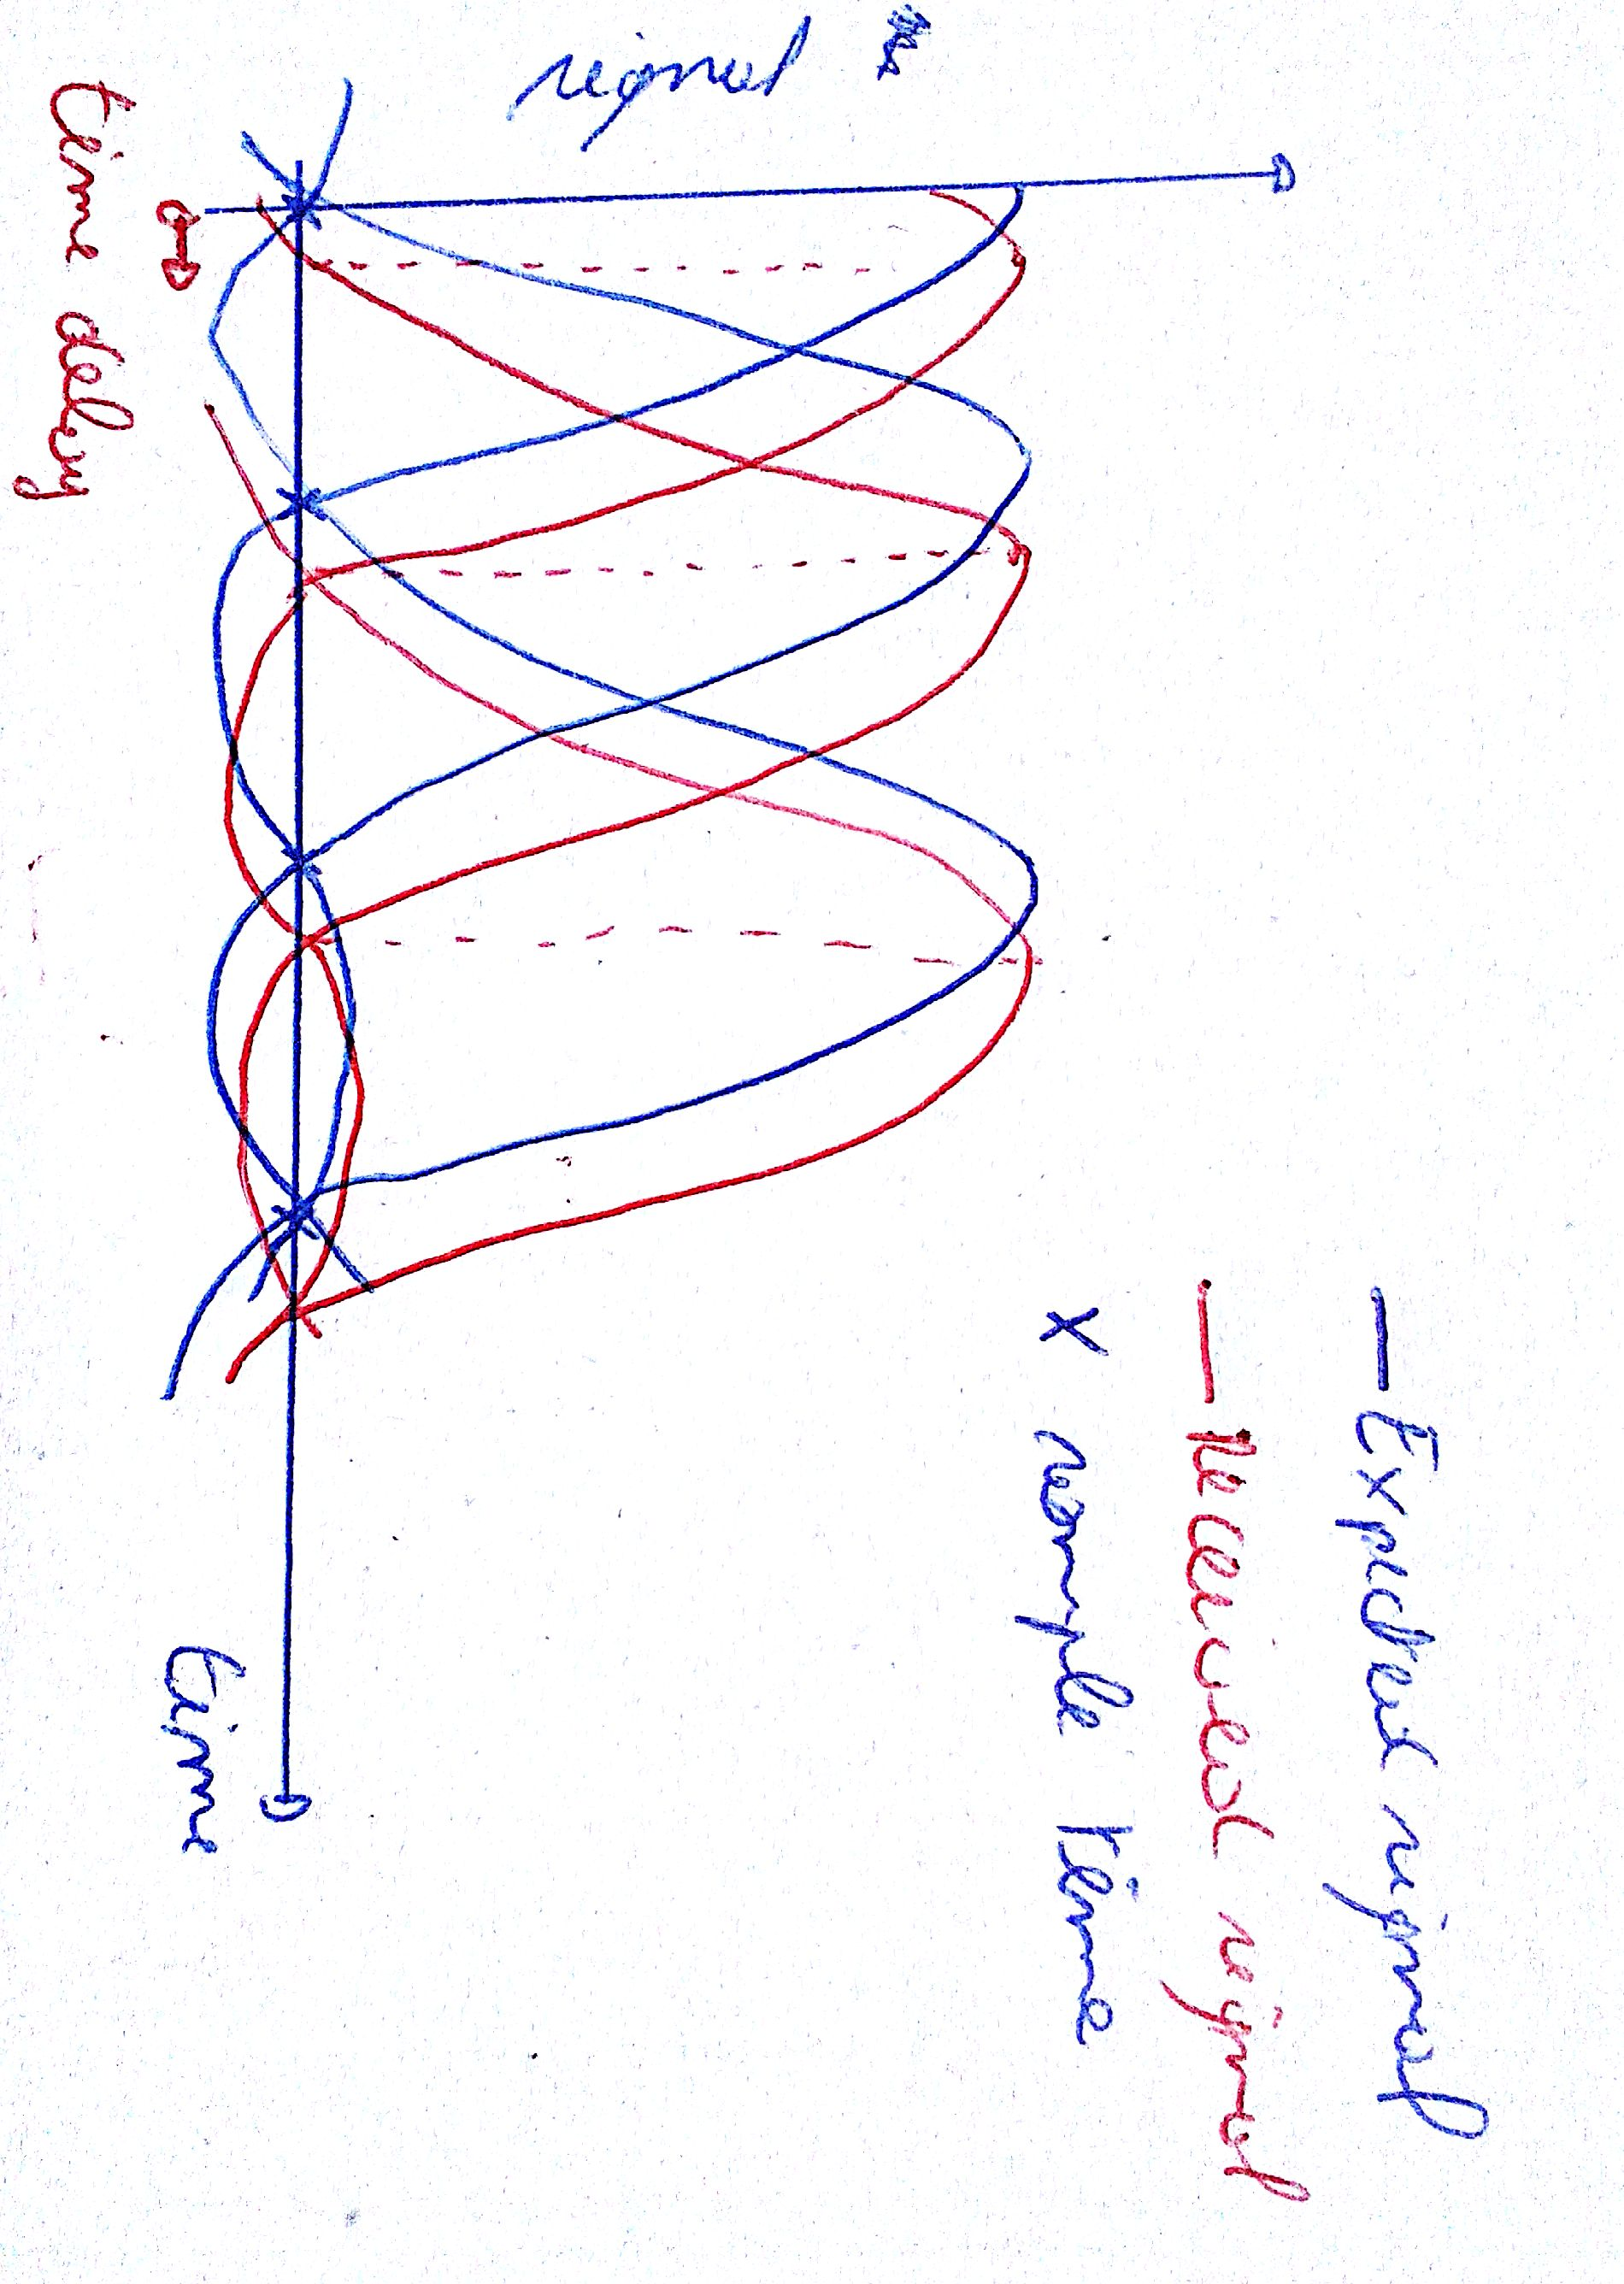
\includegraphics[width = 0.3 \textwidth , angle=90]{freq.jpg} \\
    \end{tabular}
    \caption{Similarity between frequency offset in OFDM and delay in single carrier modulation}
    \label{compare}
    \end{figure}
    
    The influence of frequency offset can be show in Figure \ref{50} and \ref{100}. Remark that a greater frequency offset means more inter carrier interference.
    \begin{figure}[h!]
        \centering
        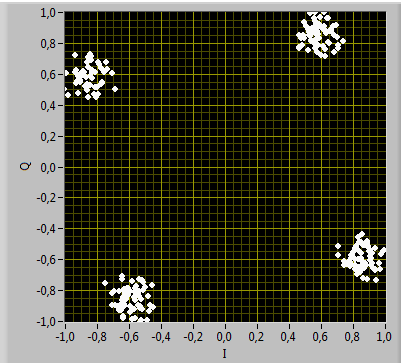
\includegraphics[width = 0.3 \textwidth]{off50_1024.PNG}
        \caption{Received constellation with frequency offset of 50 Hz}
        \label{50}
    \end{figure}
    \begin{figure}[h!]
        \centering
        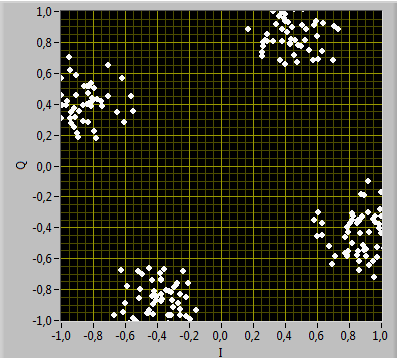
\includegraphics[width = 0.3 \textwidth]{off100_1024.PNG}
        \caption{Received constellation with frequency offset of 100 Hz}
        \label{100}
    \end{figure}
    In single carrier modulation a frequency offset cause the constellation to "smears" while in OFDM the frequency offset cause the constellation to rotate. 
    
    \subsection*{Influence of the number of subcarrier}
    We did some experiments with the same bandwidth. The given bandwidth is given by
    $$  BW = \frac{TX}{TX oversampling factor} = 0.5MHz$$
        
    We can recover the subcarrier spacing by using
    $$ \Delta _c = \frac{BW}{N}$$
        
    Where is the number of subcarrier. We did experiments for N=64 and N = 1024 so $\Delta_c$ was equal to  7812.5Hz and 488.28Hz, respectively.
    
    Because with N=1024 the symbols are less spaced in frequency domain, the same frequency offset cause more troubles (inter carrier interference and phase shift) than with N=64 (Figure \ref{fber}). This is exactly the same than for single carrier modulation with a delay : delay becomes a greater issue if the symbols are sent rapidly one after another.
    
   \begin{figure}[h!]
        \centering
        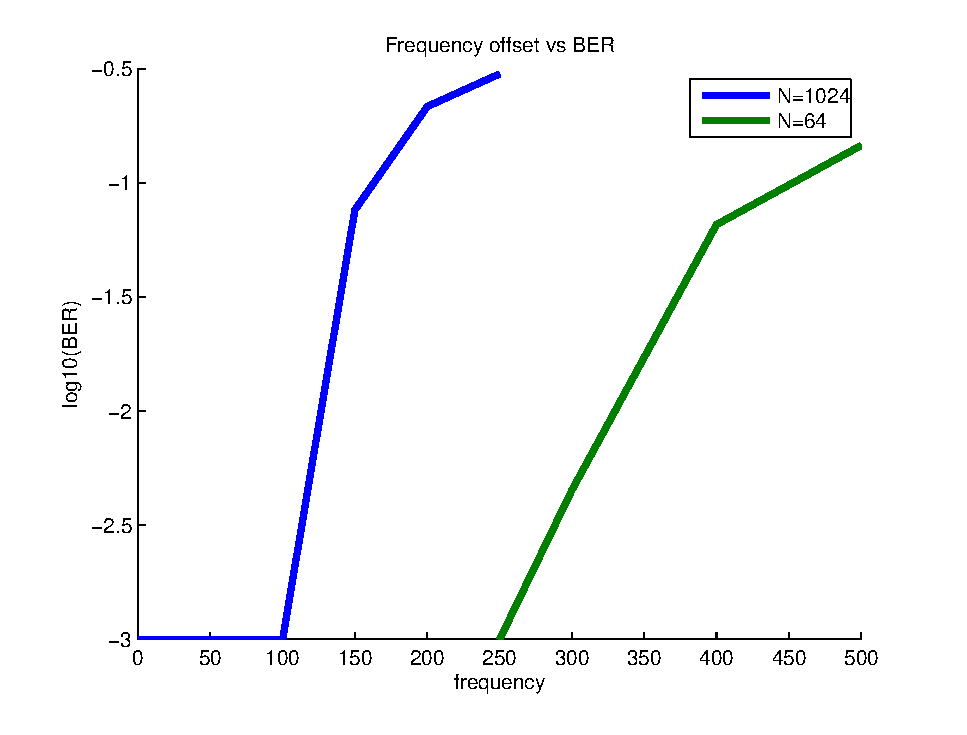
\includegraphics[width = 0.5 \textwidth]{fber.eps}
        \caption{Frequency offset vs BER for N=64 and N=1024}
        \label{fber}
    \end{figure}
        
        
\section{Lab turn in}
Because of the null tones, we send only $N-K$ symbols instead of $N$. Because of the cyclic prefix, we send those $N-K$ symbols during $N+L_c$ symbol durations, or $(N+L_c)T$ seconds; under those definitions, the effective data rate is thus equal to :
\begin{equation}
\frac{N-K}{(N+L_c)T}
\end{equation}
 
The OFDM system is especially useful in wideband systems, because it counters the frequency selectivity of those types of channels while conserving the good data rate. For narrowband systems, OFDM is more dangerous to use, because the subcarrier spacing will decrease and the system will be even more sensible to frequency offsets. Degrees of flexibility of OFDM systems include : the FFT size (or number of blocks) $N$ : increasing this number allows to make the channel "less frequency selective" for each subcarrier, but increases the sensibility to frequency offsets. Another parameter is the cyclic prefix length $L_c$ : to avoid interference, it must be at least equal to the channel response length; increasing $L_c$ allows to estimate the channel a little better, at the cost of a diminished data rate.

The bandwith is also a parameter of the OFDM modulation. Increasing the bandwith and using the same $N$ will decrease the frequency offset and ICI influence. But each subcarrier will get a more frequency selective channel.

% trouver un troisieme parametre bien
    
\end{document}
